\documentclass[10pt]{article}
\usepackage[margin=1.5cm]{geometry}
\usepackage{graphicx,hyperref,booktabs,amsmath,amssymb}
\hypersetup{colorlinks=true,urlcolor=blue}
\setlength{\parindent}{0pt}
\setlength{\parskip}{6pt}
\begin{document}
\begin{center}
{\Large P-256 regularity-halving goal: component certificates}\\[4pt]
17 November 2026 \quad Draft PR4567 \quad Unsigned producer evidence
\end{center}

The existing depth-4 full-fibre membership ideal has regularity16 in its
dense presentation and5 in the quadratic tower. The actual retained-base
control is9 versus5, below the requested twofold reduction. Complete
relation-system regularity remains unmeasured; the goal is active.

Target curve: \texttt{icv1-fp256-t89188191154553853111372247798585809583-f188c491}.
Factor base: \texttt{FB1h2704fe49495e}. Actual P-256 field; existing auxiliary
curve $w^2=x^3-3x$, using only its cyclic2-smooth subgroup. No target-log
transport is asserted.

\textbf{Definition and derivation.}
$D(J)=\operatorname{reg}(J)=\operatorname{reg}(S/J)+1$ for the homogeneous
ideal module. Homogenize the stated generators, retaining infinity
contributions. Distinguish saturation, affine final basis degree and F4
matrix degree. The tower's leading monomials are pairwise coprime squares;
the exact CI Koszul resolution gives quotient regularity$d$ and $D=d+1$.
Dense full-fibre membership has one degree$2^d$ equation. Appending the
target cubic is a regular element and increases regularity by2.

\begin{center}
\begin{tabular}{rrrrr}
\toprule
Depth & Full/retained abscissae & Membership $D$: full/kept/tower & With cubic $D$\\
\midrule
1 & 2/1 & 2/1/2 & 4/3/4\\
2 & 4/2 & 4/2/3 & 6/4/5\\
4 & 16/9 & 16/9/5 & 18/11/7\\
\bottomrule
\end{tabular}
\end{center}
Exact CI-derived values, one existing fixture per depth, no statistical or
timing data. Three native certificates and eleven corrupt-certificate
rejections; file hashes and overwrite refusal checked. Claims
\texttt{PCC-20261117-ceb084} and \texttt{ba0875}, unverified standing.

\begin{center}
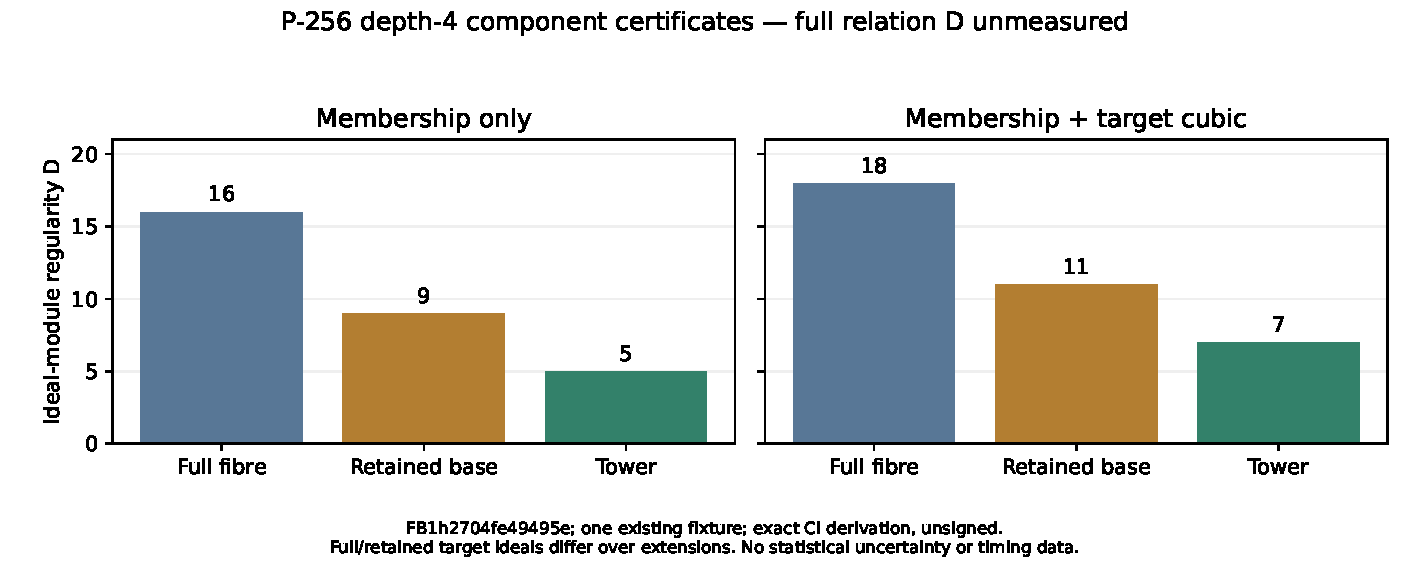
\includegraphics[width=0.97\linewidth]{components.pdf}
\end{center}

Seven depth-4 full-fibre abscissae have no target ordinate over $\mathbb F_p$
but acquire ordinates over extensions. Full and retained target ideals
therefore differ geometrically. The full-fibre ratio cannot stand in for
a matched retained-base result. Adding group-law charts and a target
changes the ideal; component regularity supplies no full-system bound.

\newpage
\textbf{Correspondence and unresolved obligation}
\begin{center}
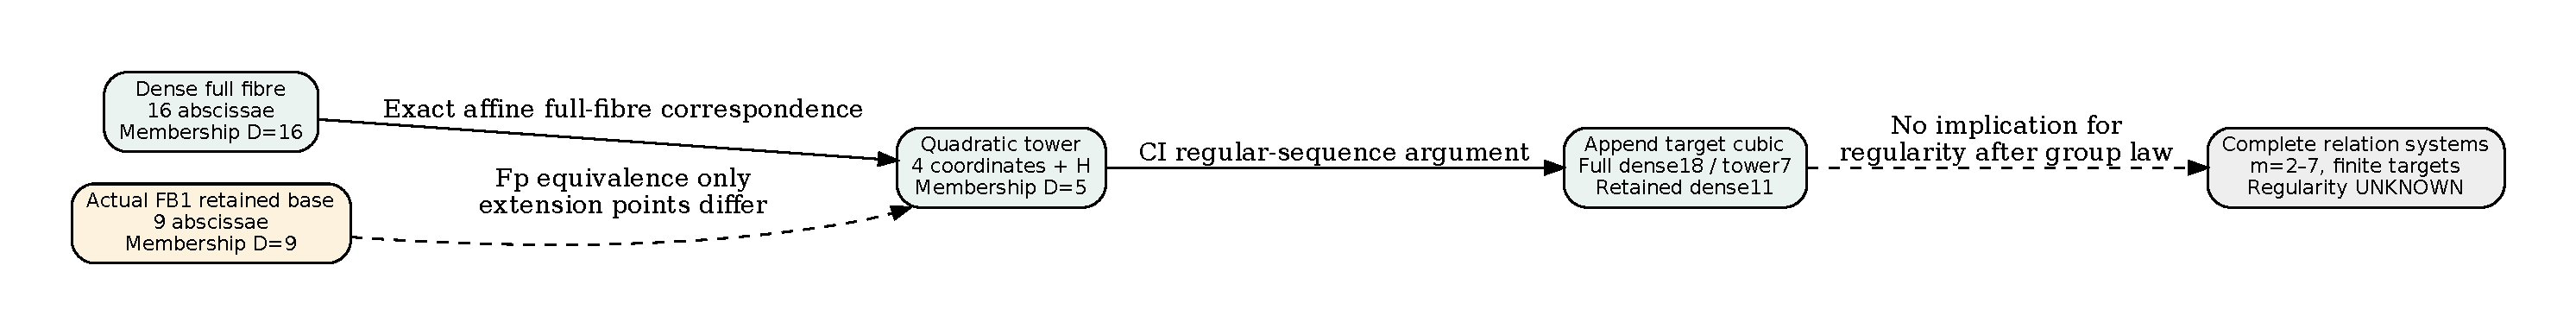
\includegraphics[width=\linewidth]{obligations.pdf}
\end{center}

\textbf{Complete-system qualification.}
An exact native exporter applies the same constant-pivot linear
preprocessing to dense and tower arms. It checks coefficientwise that
$H=1$ recovers each residual generator, and emits original/residual
systems and reconstruction certificates for finite planted depth2/4
$m=2$ targets. Programs22497/27709 bytes were published before submission.
This small qualification does not discharge $m=2$--7 or depth8.

\begin{itemize}
\item Request001 returned HTTP200 but success=false/exit1: the public
Magma service forbids \texttt{Alarm(20)}. Execution stopped before the CI
probe. Full raw input/response retained.
\item The explicitly amended final request removed only that control
line. The disclosed limit became the service300-second cap plus a25-second
HTTP deadline. The client timed out after25003ms with zero received bytes,
curl28. Remote outcome unknown; no result admitted and no retry.
\end{itemize}

Both requests consumed the frozen allowance. Depth4 was not submitted.
These failures establish no mathematical obstruction. No new relation was
reported, so none could be replayed from these requests. Prior continuation
replays remain unchanged. Claims \texttt{a7e5de}, \texttt{19ac2d} and
\texttt{3b7fda} preserve the failure and prospective correction records.

\textbf{Reproduce.}
Run \texttt{run\_checks.sh FRESH\_DIR} for native exact component checks
and byte replay; \texttt{build\_complete.sh FRESH\_DIR} reconstructs frozen
CAS inputs. Neither submits a network request. C++20/O2/Wall/Wextra/Werror,
GMP/OpenSSL; local development, no performance admission. Original failed
native source, compiler log and successor correction are retained.

The companion \texttt{IDC1hfd07bef9fab74b95} samples the universal quadratic
expansion under the repository's fixed $2^{61}-1$ identity schema, with a
separate exact P256 coefficient check. The official Rust checker was
unavailable; no Lean or independent signed theorem is claimed.

\textbf{Next obligation.}
A runnable exact graded-resolution verifier must supply the missing
complete-system regularity certificate, first on the frozen finite depth4
cell, then across the original $m=2$--7/depth8 workload. Count all extra
variables and covers; retain the actual-base challenger and exact replay.
Do not infer runtime or novelty from local degree. PR4567 stays draft.

\textbf{Evidence and sources.}
See \texttt{REPORT.md}, \texttt{PROOF.md}, protocols/amendments and
\texttt{evidence/native}, \texttt{evidence/api001}, \texttt{evidence/api002}.
Magma's official free-resolution manual documents
\texttt{QuotientModule}/\texttt{Regularity}; Macaulay2 documents the
ideal/quotient offset. PKC2016 auxiliary-isogeny prior art is linked in
\texttt{PROTOCOL.md}. KB retrieval and conductor were unavailable. All
mathematical/result claims here have unsigned producer standing only.
\end{document}
